\section[网中的零空间]{网中的零空间\\Nullspaces for Networks}	
\par \noindent
%\emph{水准网(一维,只有高程)}。关联矩阵取不同的高程。零空间包含着等高向量:
水准网(一维,只有高程)。关联矩阵取不同的高程。零空间包含着等高向量:
\begin{equation}
	e =
	\begin{pmatrix}
		1,1,...,1
	\end{pmatrix}
\end{equation}
%\emph{二维控制网$A$ }在$x$方向上平移,给所有的$x$坐标增加了一个常数。在二维空间中,也有一次在y轴方向上的平移和一个刚性平移。如果未知向量如下:
二维控制网$A$在$x$方向上平移,给所有的$x$坐标增加了一个常数。在二维空间中,也有一次在y 轴方向上的平移和一个刚性平移。如果未知向量如下:
\begin{equation}
	X =
	\begin{pmatrix}
		X_1,Y_1,X_2,Y_2,...,X_n,Y_n
	\end{pmatrix}
\end{equation}
A的零空间包括$x$和$y$的平移:
\begin{equation}
	t_x =
	\begin{pmatrix}
		1,0,1,0,...,1,0
	\end{pmatrix}
	\  \text{和}\   t_y =
	\begin{pmatrix}
		0,1,0,1,...,0,1
	\end{pmatrix} \text{。}
\end{equation}
%而且网可以\emph{旋转}一个角度$φ$。我们将详细显示如何线性化一次微分旋转:
而且网可以旋转一个角度$φ$。我们将详细显示如何线性化一次微分旋转:
\begin{align}
	\begin{split}
		X_{i}^{'} = cos{\varphi}X_i - sin{\varphi}Y_i \\
		Y_{i}^{'} = sin{\varphi}X_i + cos{\varphi}Y_i
	\end{split}
\end{align}
这里$(X_i,Y_i)$是一组所给坐标,经过旋转转换为$(X_{i}^{'}, Y_{i}^{'})$。我们通过$\sin d\varphi \approx 1$ 、$\cos d\varphi \approx 1$进行线性化并且只保留一阶,得到:
\begin{align*}
	X_{i}^{'} + \varepsilon_i = 1 X_i - d\varphi Y_i\qquad  \varepsilon_i = -Y_i d\varphi   \\
	Y_{i}^{'} + \eta_i = d\varphi X_i + 1 Y_i\qquad
	\eta_i = X_i d\varphi \text{。}
\end{align*}
这个旋转量虽然小但在$A$的零空间中产生了另外一个向量:
\begin{equation}
	\mathbf{r_{\varphi}} =
	\begin{pmatrix}
		-Y_1,X_1,-Y_2,X_2,...,Y_n,X_n
	\end{pmatrix} \text{。}
\end{equation}
% 最终\emph{在$dk$尺度上的改变}通过这个向量描述:
最终在$dk$尺度上的改变通过这个向量描述:
\begin{equation}
	s_k =
	\begin{pmatrix}
		X_1,Y_1,X_2,Y_2,...,X_n,Y_n
	\end{pmatrix} \text{。}
\end{equation}
我们通过两次平移,一次旋转,一次尺度改变确定了控制网。
\par\noindent
零空间$N(A)$由下面四行组成
\begin{equation}
	G^T =
	\begin{bmatrix}
		\color{red} 1&0&1&0&...&1&0\\
		0&1&0&1&...&0&1\\
		-Y_1&X_1&-Y_2&X_2&...&Y_n&X_n\\
		X_1&Y_1&X_2&Y_2&...&X_n&Y_n
	\end{bmatrix} \text{。}
\end{equation}
微分参数是$df = (dt_x,dt_y,d\varphi,dk)$,平移参数是
\begin{equation}
	dx =
	\begin{pmatrix}
		\xi_1,\eta_1,...,\xi_n,\eta_n
	\end{pmatrix}
	= Gdf \text{。}
\end{equation}
\textbf{例7.1}  (距离测量)我们为了确定点$P$观测了三段距离:
\begin{equation}
	f_1 = 100.01\qquad \qquad f_2 = 100.02\qquad \text{和}\qquad f_3 = 100.03
\end{equation}
权重$C = \text{diag}(1,1,1) = I$。图7.1标示了所有坐标的初始值。作为点P的初始坐标,我们使用$(X_{P}^{0},Y_{P}^{0}) = (170.71, 170.71)$。这些值是通过简单的几何关系被计算出来。
\begin{figure}
	\centering
	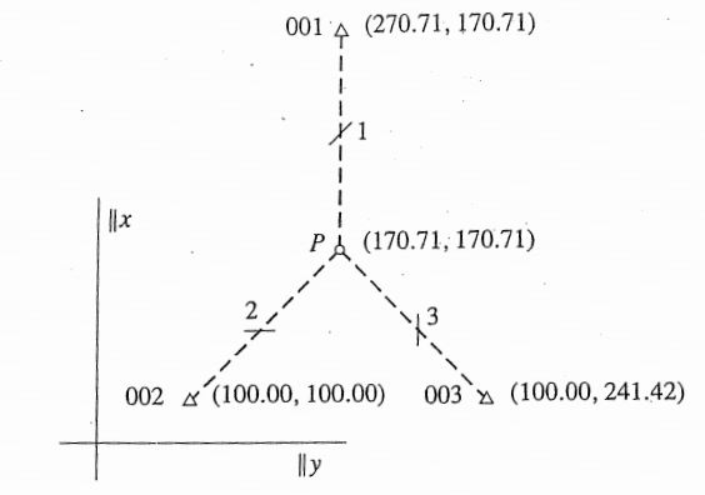
\includegraphics[width=0.4\linewidth]{TeX_files/Part02/chapter07/image/7-1}
	\caption{图7.1   通过后方交会确定一个点的坐标}
	\label{fig:7-1}
\end{figure}

\par
第一个观测方程是
\begin{equation*}
	\begin{bmatrix}
		- cos{\alpha_{P,001}^{0}} & - sin{\alpha_{P,001}^{0}}
	\end{bmatrix}
	\begin{bmatrix}
		x_P \\ y_P
	\end{bmatrix}
	= f_1 - \sqrt{(X_{001}^{0} - X_{p}^{0})^2 + (Y_{001}^{0} - Y_{p}^{0})^2} - e_1
\end{equation*}
或者
\begin{equation*}
	\begin{bmatrix}
		-1 & 0
	\end{bmatrix}
	\begin{bmatrix}
		x_P \\ y_P
	\end{bmatrix}
	= f_1 - 100.000 - e_1 \text{,}
\end{equation*}
同样地,第二个观测方程是
\begin{equation*}
	\begin{bmatrix}
		0.707 1 & 0.7071
	\end{bmatrix}
	\begin{bmatrix}
		x_P \\ y_P
	\end{bmatrix}
	= f_2 - 99.999 - e_2 \text{,}
\end{equation*}
最后第三个观测方程是
\begin{equation*}
	\begin{bmatrix}
		0.707 1 & -0.7071
	\end{bmatrix}
	\begin{bmatrix}
		x_P \\ y_P
	\end{bmatrix}
	= f_3 - 99.999 - e_3 \text{。}
\end{equation*}
现在三个观测方程组在一起为
\begin{equation*}
	\begin{bmatrix}
		-1 & 0\\
		0.707 1 & 0.7071\\
		0.707 1 & -0.7071
	\end{bmatrix}
	\begin{bmatrix}
		\hat{x}_P \\ \hat{y}_P
	\end{bmatrix}
	= \begin{bmatrix}
		100.01- 100.000\\
		100.02- 99.999\\
		100.03- 99.999
	\end{bmatrix}
	-
	\begin{bmatrix}
		e_1\\
		e_2\\
		e_3
	\end{bmatrix}
\end{equation*}
法方程$A^\mathsf{T}A\hat{x} = A^\mathsf{T}b$是
\begin{equation*}
	\begin{bmatrix}
		2  & 0 \\
		0 & 1
	\end{bmatrix}
	\begin{bmatrix}
		\hat{x}_P \\ \hat{y}_P
	\end{bmatrix}
	=
	\begin{bmatrix}
		0.0267\\
		-0.0071
	\end{bmatrix} \text{。}
\end{equation*}
由于系数阵变成了对角阵(为什么$A^\mathsf{T}A$在这种情况中是对角阵?),所以很容易得到$(\hat{x}_P,\hat{y}_P) = (0.013 4,-0.007 1)$。最终坐标$(\hat{X}_P,\hat{Y}_P) = (X_{P}^{0} +
\hat{x}_P,Y_{P}^{0} + \hat{y}_P =  (170.723 m, 170.703 m))$。
\par
在这个简单例子中,残差是最容易被计算的:
\begin{equation*}
	\hat{e} = b - A\hat{x}
	= b - P
	=
	\begin{bmatrix}
		0.01 \\ 0.02 \\ 0.03
	\end{bmatrix}
	-
	\begin{bmatrix}
		-0.0127 \\ 0.0040 \\ 0.0140
	\end{bmatrix}
	=
	\begin{bmatrix}
		0.0234 \\ 0.0165 \\ 0.0165
	\end{bmatrix} \text{。}
\end{equation*}
最终${\hat{\sigma}}_0 = \sqrt{\hat{e}^\mathsf{T}\hat{e}/(3 - 2)} = 0.033m$。协方差为:
\begin{equation*}
	\Sigma_{\hat{x}}
	= {\hat{\sigma}}_{0}^{2}(A^\mathsf{T}A)^{-1}
	=
	\begin{bmatrix}
		0.000514 & 0\\
		0 & 0.001029
	\end{bmatrix}
\end{equation*}
坐标的标准偏差为$\sigma_{\hat{X}_P} = \sqrt{0.000514} = 0.023$米和$\sigma_{\hat{X}_P} = \sqrt{0.001 029} = 0.033$米。
\par\noindent
%\emph{三维控制网} 三维网受三个无穷小平移量$dt_x,dt_y,dt_z$、三个无穷小旋转量$d\varphi_x,d\varphi_y,d\varphi_z$、一个尺度改变量$dk$控制。空间向量是以下七行:
三维控制网 三维网受三个无穷小平移量$dt_x,dt_y,dt_z$、三个无穷小旋转量$d\varphi_x,d\varphi_y,d\varphi_z$、一个尺度改变量$dk$控制。空间向量是以下七行:
\begin{equation}
	G^\mathsf{T}
	=
	\begin{bmatrix}
		1 & 0 & 0 \\
		0 & 1 & 0 \\
		0 & 0 & 1 \\
		0 & -Z_1 & Y_1 \\
		Z_1 & 0 & -X_1 \\
		-Y_1 & X_1 & 0 \\
		X_1 & Y_1 & Z_1
	\end{bmatrix}
	\cdots
	\begin{bmatrix}
		1 & 0 & 0 \\
		0 & 1 & 0 \\
		0 & 0 & 1 \\
		0 & -Z_n & Y_n \\
		Z_n & 0 & -X_n\\
		-Y_n & X_n & 0 \\
		X_n & Y_n & Z_n
	\end{bmatrix}
\end{equation}
其中,
\begin{equation}
	df
	=
	\begin{pmatrix}
		dt_x,dt_y,dt_z,d\varphi_x,d\varphi_y,d\varphi_z \\
	\end{pmatrix}
\end{equation}
$G$的列($G^\mathsf{T}$的行)跨越了$N(A)$,我们得到
\begin{equation}
	AG = 0 \text{。}
\end{equation}
我们通过提出一个几何解释结束本节。$G^\mathsf{T}x = 0$的前三行表示原点是固定的。由于数值原因,我们将原点平移到重心,并且提供了与重心有关的坐标
$(X^\ast,Y^\ast,Z^\ast)$:
\begin{equation*}
	\sum_{i=1}^{n}X^\ast = 0,\qquad\sum_{i=1}^{n}Y^\ast = 0,\qquad\sum_{i=1}^{n}Z^\ast = 0 \text{。}
\end{equation*}
下面的三个公式$G^\mathsf{T}x = g$ 导致旋转:
\begin{equation*}
	\sum_{i=1}^{n}(-Y_{i}^{\ast}\varepsilon_i + X_{i}^{\ast}\eta_i) = g_4,\qquad
	\sum_{i=1}^{n}( Z_{i}^{\ast}\varepsilon_i - X_{i}^{\ast}\zeta_i) = g_5\qquad
	\sum_{i=1}^{n}(-Z_{i}^{\ast}\eta_i        + Y_{i}^{\ast}\zeta_i) = g_6 \text{。}
\end{equation*}
最后的条件$\sum_{n=1}^n(X_{i}^{\ast}\varepsilon_i + Y_{i}^{\ast}\eta_i + Z_{i}^{\ast}\zeta_i)$保证尺度是固定的。
\par\noindent
\textbf{表 7.1}  %生成A的零空间的可能的G列伊尼森。
在每个节点的未知数用$u$标示,$d$是$N(A)$的维数。
\begin{center}
	\begin{tabular}{cccccccccc}
		\hline
		\multirow{2}{*}{$u$}& \multirow{2}{*}{$d$} & \multirow{2}{*}{观测值类型(s)} & \multicolumn{7}{c}{$G$列组成部分(s)} \\
		\cline{4-10}
		\multicolumn{3}{c}{}    &  \multicolumn{3}{c}{平移(s)} &  \multicolumn{3}{c}{旋转 (s)} & 尺度(s)\\
		\hline
		1 & 1 &高差 & &1\\
		\hline
		\multirow{2}{*}{} & \multirow{2}{*}{2}  & \multirow{2}{*}{距离和方位角} &1&0\\
		\multicolumn{3}{c}{} &0&1\\
		\\
		\multirow{2}{*}{2} & \multirow{2}{*}{3} & \multirow{2}{*}{距离} &1 &0&&& \quad$Y_i$\\
		\multicolumn{3}{c}{} &0&1&&& $-X_i$\\
		\\
		\multirow{2}{*}{} & \multirow{2}{*}{4} & \multirow{2}{*}{角度和或者距离比率} &1 &0&&& \quad$Y_i$ &&$X_i$\\
		\multicolumn{3}{c}{} &0&1&&& $-X_i$&&$Y_i$\\
		\hline
		\multirow{3}{*}{} & \multirow{3}{*}{3} & 距离, 方位角, &1&0&0\\
		\multicolumn{2}{c}{} &天文纬度 和&0&1&0\\
		\multicolumn{2}{c}{} &经度&0&0&1\\
		\\
		\multirow{3}{*}{3} & \multirow{3}{*}{6} & \multirow{3}{*}{距离} &1&0&0 &\quad0&$-Z_i$&\quad$Y_i$\\
		\multicolumn{3}{c}{} &0&1&0&\quad$Z_i$&\quad0&$-X_i$\\
		\multicolumn{3}{c}{} &0&0&1&$-Y_i$&\quad$X_i$&\quad0\\
		\\
		\multirow{3}{*}{} & \multirow{3}{*}{7} & \multirow{3}{*}{角度和或者距离比率} &1&0&0 &\quad0&$-Z_i$&\quad$Y_i$&$X_i$\\
		\multicolumn{3}{c}{} &0&1&0&\quad$Z_i$&\quad0&$-X_i$&$Y_i$\\
		\multicolumn{3}{c}{} &0&0&1&$-Y_i$&\quad$X_i$&\quad0&$Z_i$\\
		\hline
	\end{tabular}
\end{center}


\backmatter
% bibliography, glossary and index would go here.